\chapter{Testing}%%%%%%%%%%%%%%%%%%%%%%%%%%%%%%%%%%%%%%%%%%%%%% 
\label{chap:testing}

In this chapter the various software implementations and design choices made in \refchap{chap:implementation} are used and tested on various aspects. 
This is done to gather the data needed to answer the second, third and fourth research question. 
It consists of the sections \refsec{sec:testing:compilation} and \refsec{sec:testing:usability}.


\section{Plugin Compilation Tests}
\label{sec:testing:compilation}

\subsection{Rust: minimal plugin}
The compilation of a minimum Rust plugin, exposing a function, a class, and a method was successful. 
% APPENDIX?
\reffig{fig:min-rust-plugin-code:1} Shows the source code of this plugin. 
The 'wasm-bindgen' library allows functions and classes to be annotated as 'bound to javascript'. 
This simplifies the compilation process to WebAssembly greatly. 
It also clearly states errors if a property or class are incompatible to be exposed. 

This library was compiled to WebAssembly and javascript using 'wasm-pack'. 
This produces multiple artifacts, showcased in \reffig{fig:rust-plugin:compilation-results}. 
This figure also showcases how wasm-pack wraps the functionality: 
The \m{point\_distance} function exposed by the wasm file is wrapped by the javascript file, converting it to look like a regular javascript class.

To check if the result is valid, a small html demo was created to load and use the library (see \reffig{fig:min-rust-plugin-code:2}).
Note how the JavaScript library wrapping the wasm file looks and works almost like a normal javascript library, the only difference being a 'init' function, which is required to be run before using the library, and the need to free the memory of used object with the \m{free\(\)} method.

\begin{figure}
  \centering
  \begin{subfigure}[b]{0.45\linewidth}
    \graphicspath{{../../assets/images/6.1.1/}}
    \centering
    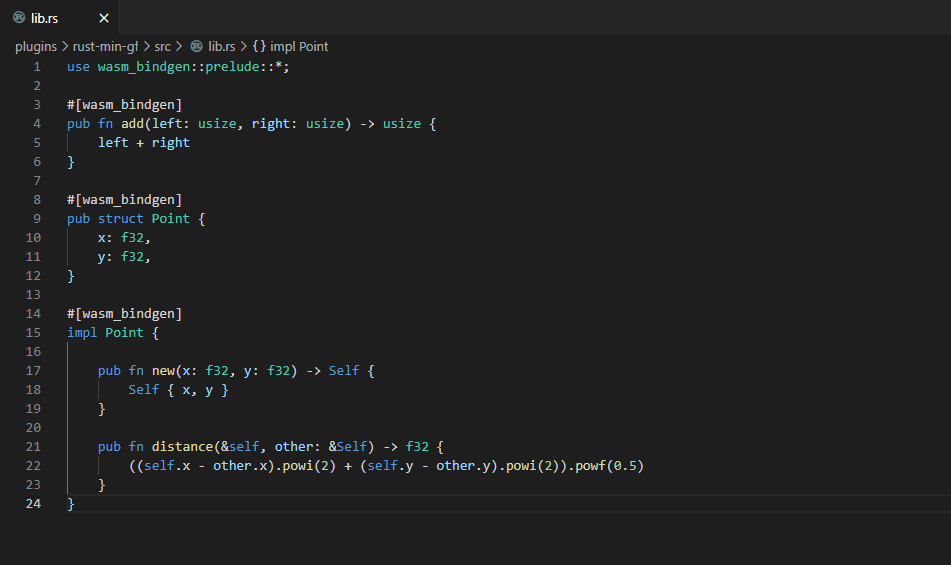
\includegraphics[width=\linewidth]{8.PNG}
    \caption{}\label{fig:min-rust-plugin-code:1}
  \end{subfigure}%
  \qquad %-- that adds some space between th 2 figures
  \begin{subfigure}[b]{0.45\linewidth}
    \graphicspath{{../../assets/images/6.1.1/}}
    \centering
    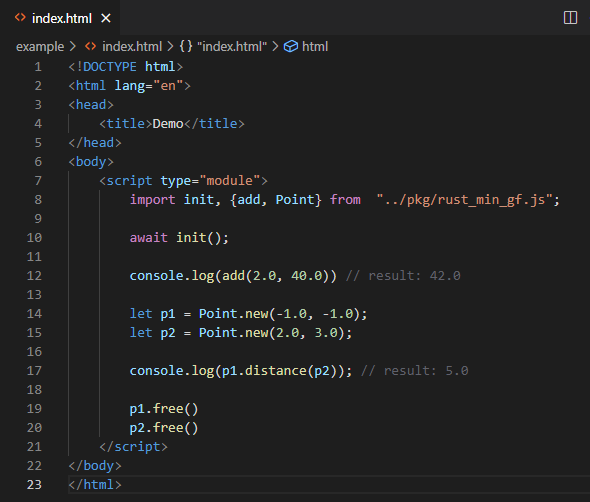
\includegraphics[width=\linewidth]{9.PNG}
    \caption{}\label{fig:min-rust-plugin-code:2}
  \end{subfigure}%
  \caption[minimal rust geofront plugin: usage]{Rust Source code (a) and web demo (b)}
  \label{fig:min-rust-plugin-code}
\end{figure}

\begin{figure}
  \graphicspath{{../../assets/images/6.1.1/}}
  \centering
  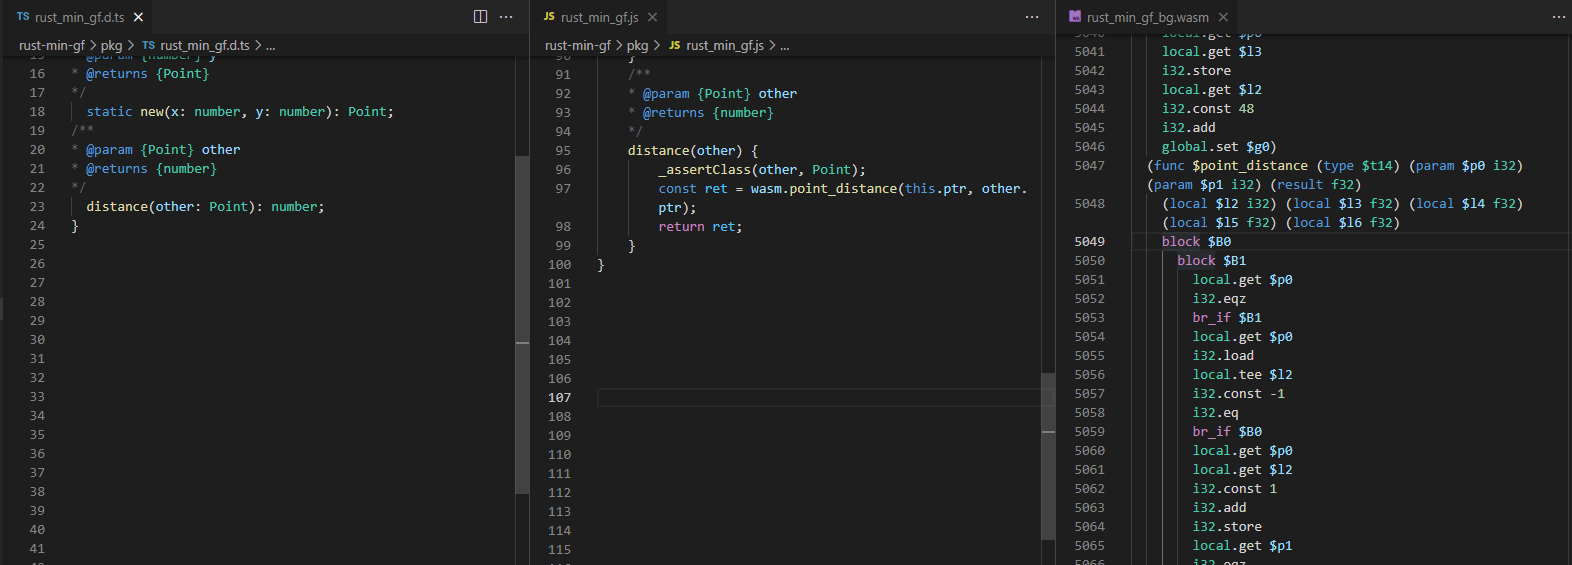
\includegraphics[width=\linewidth]{13.PNG}
  \caption[compilation artifacts]{Compilation artifacts: A Typescript Declaration file, a javascript file, and a WebAssembly binary, visualized as WebAssembly Text (WAT). }
  \label{fig:rust-plugin:compilation-results}
\end{figure}

To load this project into Geofront, a reference to the path of the compilation artifacts must be specified within the Geofront GUI, shown in \reffig{fig:min-rust-plugin-import}.
A local path was used for convenience, instead of publishing this demo to npm, and accessing it via a \ac{CDN}.

\begin{figure}
  \graphicspath{{../../assets/images/6.1.1/}}
  \centering
  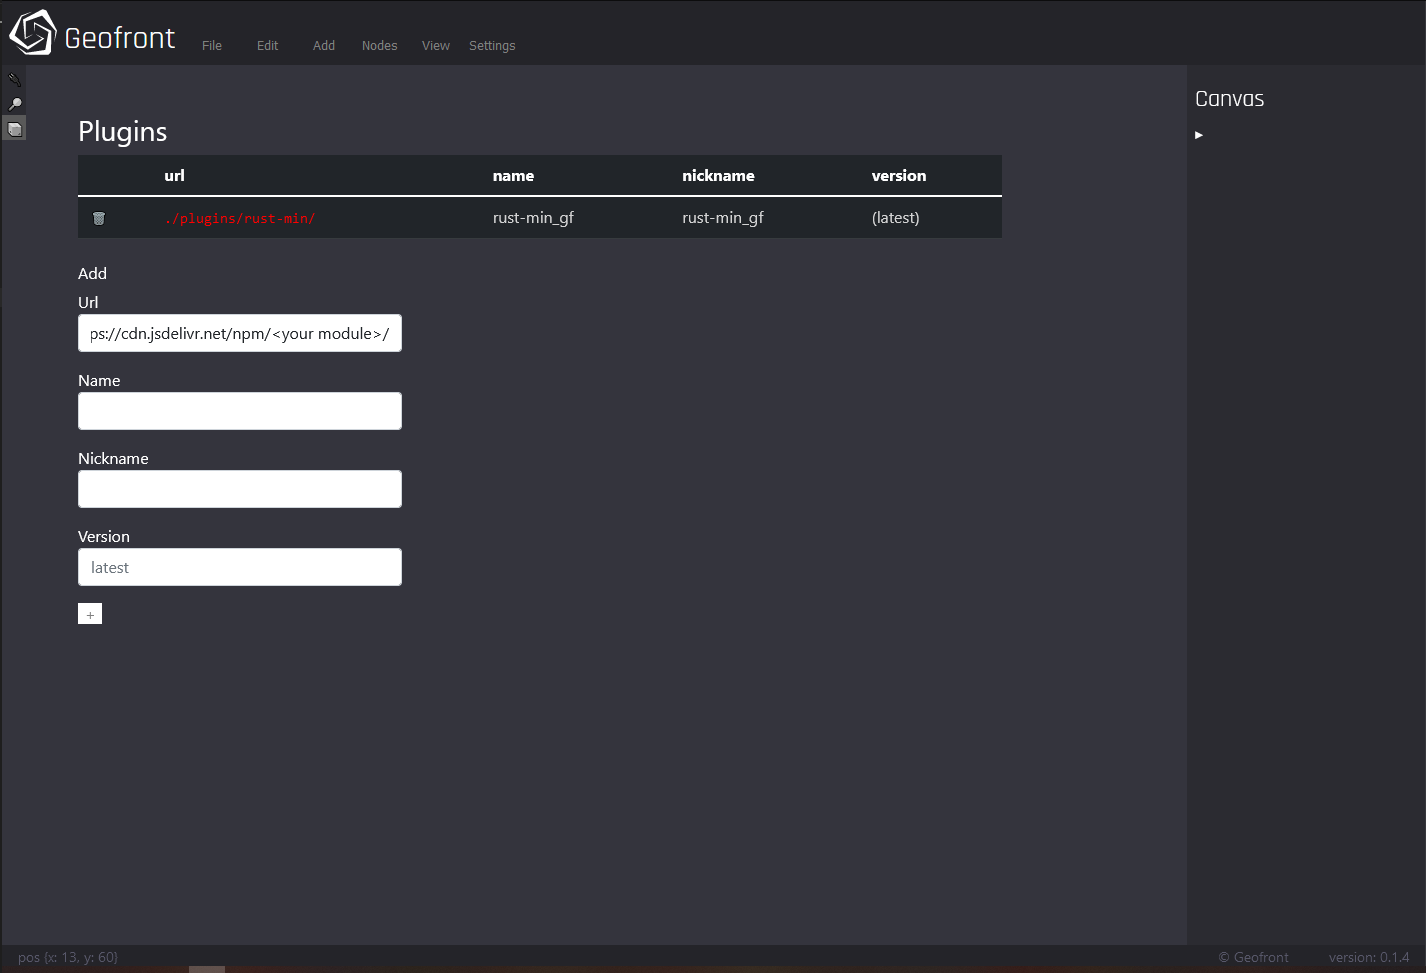
\includegraphics[width=0.50\linewidth]{2.PNG}
  \caption[loading a plugin]{Loading a plugin into Geofront using the \ac{GUI}}
  \label{fig:min-rust-plugin-import}
\end{figure}

\reffig{fig:rust-plugin-on-canvas:1} shows how all functions in this demo are loaded correctly, and \reffig{fig:rust-plugin-on-canvas:2} shows that the functions indeed work as expected to create two Graphs. 
Note how the parameter names and Types are also loaded, indicated by the names visualized at the input and output of the nodes.
This is thanks to the 'd.ts' file of \reffig{fig:rust-plugin:compilation-results}.

All in all, no problems were encountered.

\begin{figure}
  \centering
  \begin{subfigure}[b]{0.45\linewidth}
    \graphicspath{{../../assets/images/6.1.1/}}
    \centering
    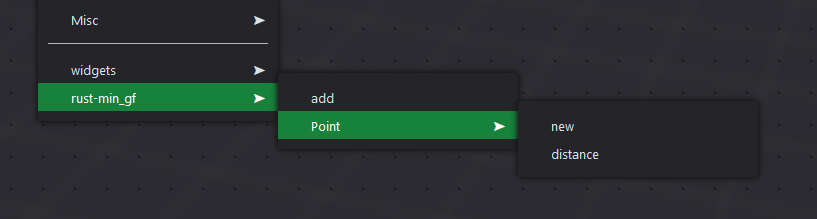
\includegraphics[width=\linewidth]{7.PNG}
    \caption{}\label{fig:rust-plugin-on-canvas:1}
  \end{subfigure}%
  \qquad %-- that adds some space between th 2 figures
  \begin{subfigure}[b]{0.45\linewidth}
    \graphicspath{{../../assets/images/6.1.1/}}
    \centering
    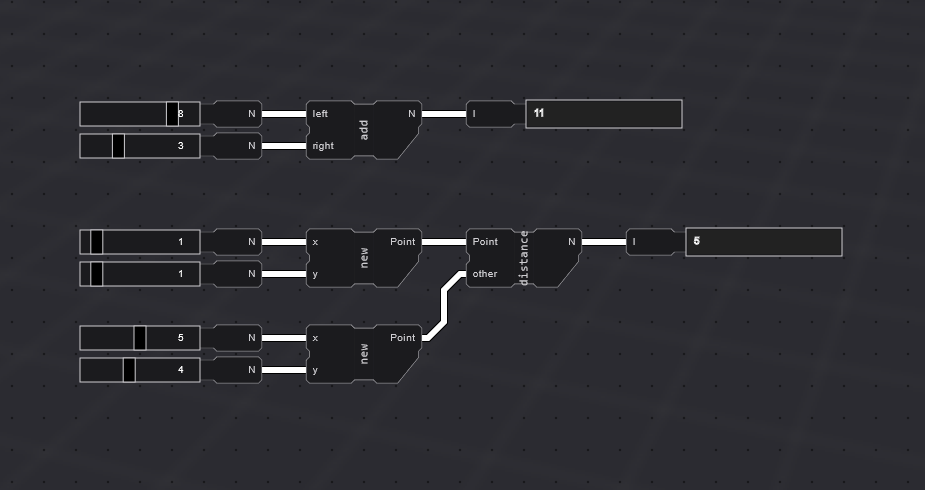
\includegraphics[width=\linewidth]{6.PNG}
    \caption{}\label{fig:rust-plugin-on-canvas:2}
  \end{subfigure}%
  \caption[minimal rust geofront plugin: usage]{Usage On the canvas}
  \label{fig:rust-plugin-on-canvas}
\end{figure}

\subsection{Rust: Startin plugin}

Compilation of the \m{Startin} library was also successful. 
Startin already offered a wasm-ready library, this could directly be loaded into Geofront. 
However, the API exposed by this library used a non-functional style, making it hard to properly use the library on a VPL canvas. 
This is why a custom plugin library still had to be created, in which functions like '\m{new\_from\_vec}' were added to support functional usage. 

Other than that, all steps performed by the minimal Rust plugin could be made with this project as well, as shown in \reffig{fig:startin-plugin}. 
This also showcases the usage of the 'Renderable' bindings. 
This way, a variable of type 'Triangulation' can be viewed in 3D by clicking on it.

\begin{figure}
  \centering
  \begin{subfigure}[b]{\linewidth}
    \graphicspath{{../../assets/images/6.1.2}}
    \centering
    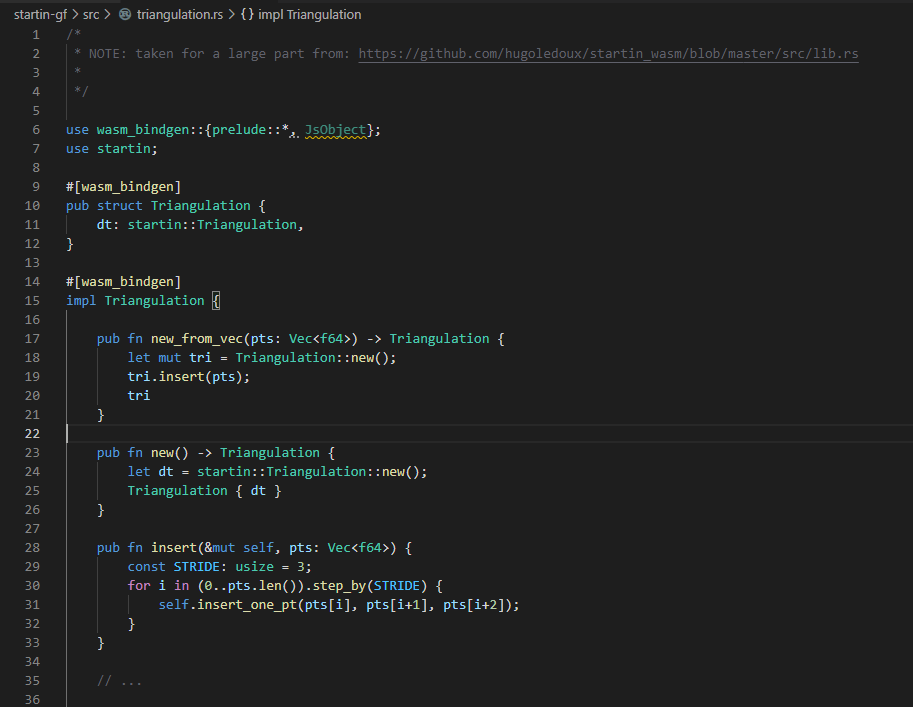
\includegraphics[width=\linewidth]{1.PNG}
  \end{subfigure}%
  \\ 
  \begin{subfigure}[b]{\linewidth}
    \graphicspath{{../../assets/images/6.1.2}}
    \centering
    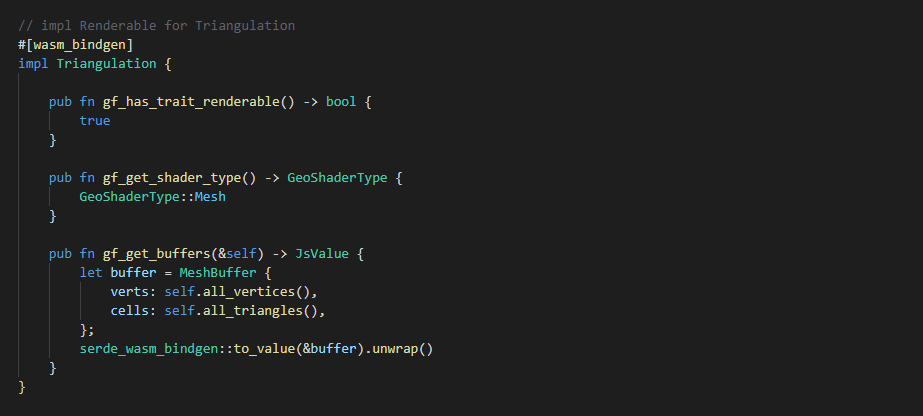
\includegraphics[width=\linewidth]{5.PNG}
  \end{subfigure}%
  \\
  \begin{subfigure}[b]{\linewidth}
    \graphicspath{{../../assets/images/6.1.2}}
    \centering
    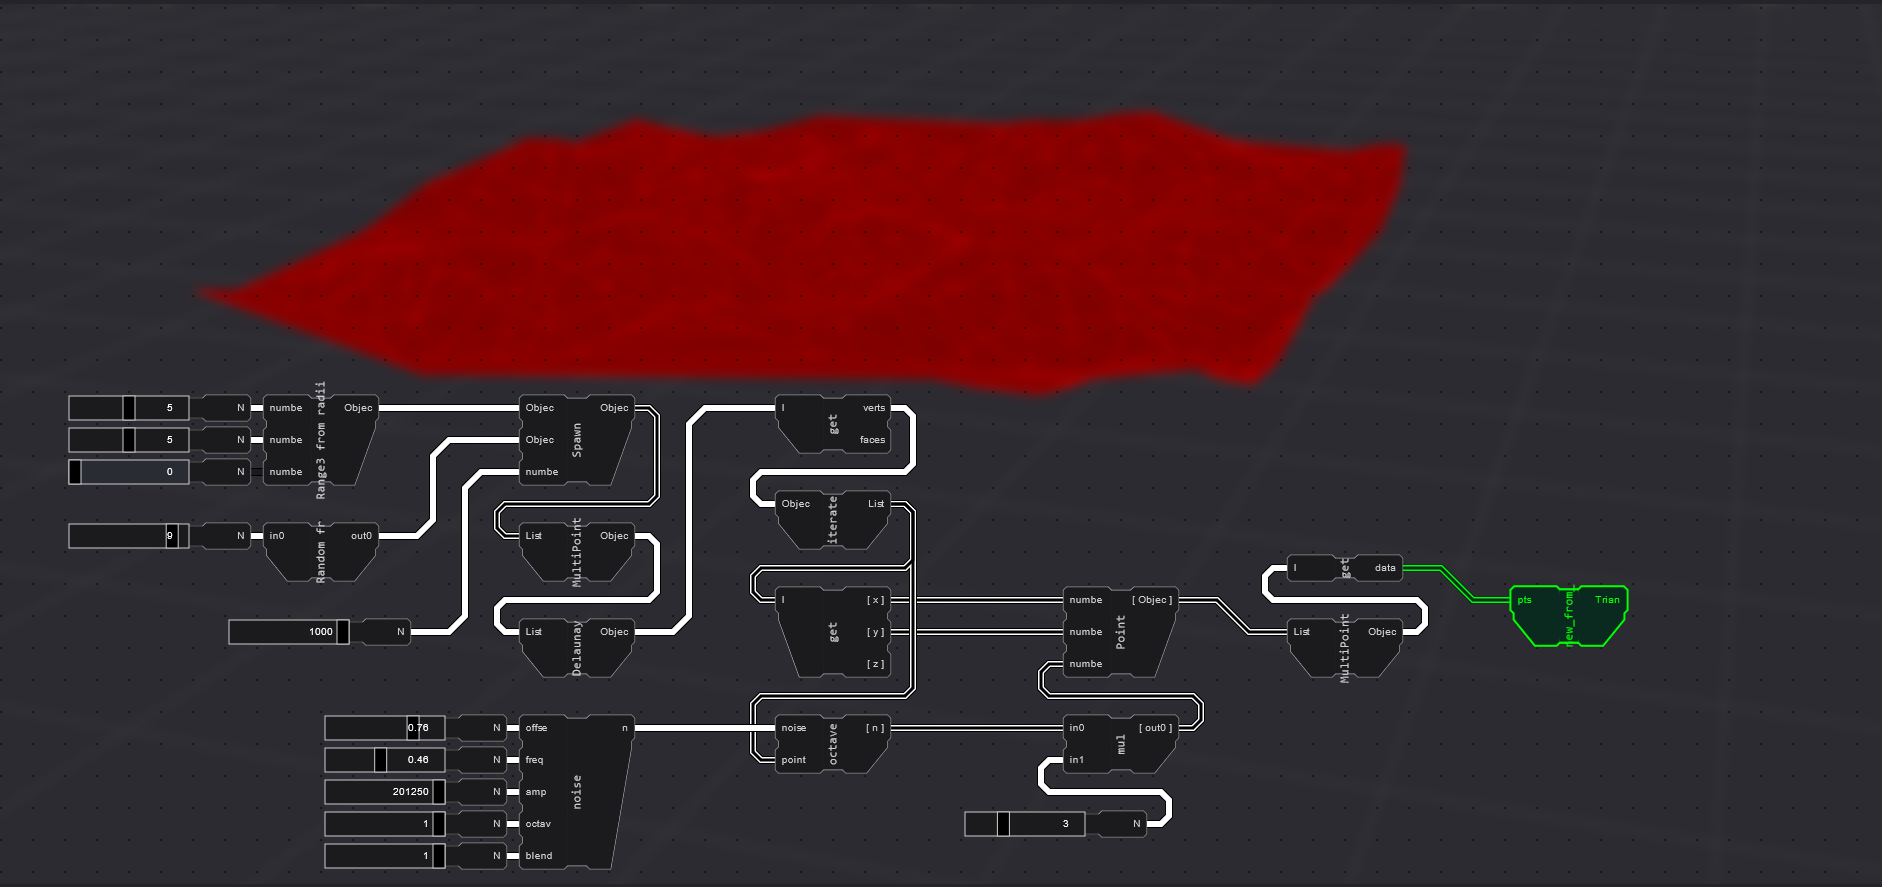
\includegraphics[width=\linewidth]{2.PNG}
  \end{subfigure}%
  \caption[Types of \ac{vpl}s]{Startin, loaded as plugin within Geofront}%
  \label{fig:startin-plugin}
  \end{figure}

\subsection{C++: Minimal plugin}  

Making a minimal C++ plugin work in a Geofront graph was unsuccessful.
It was, however, possible to compile the plugin file to WebAssembly, and to use it in a web demo, but this was not without its obstacles. 

First of all, the construction of the C++ source code itself.
Emscripten's \m{embind} tool uses a macro syntax to flag functions marked for javascript compilation, shown in \reffig{fig:min-cpp-source}. 
While it does work similar to Rusts \m{wasm_bindgen}, cpp macro's do not allow for any pre-compile-time code checking, and can produce hard to decipher error messages. 

Secondly, to compile this file to the right binary with accompanied javascript wrapper, it had to be compiled using the relatively unknown \m{-sMODULARIZE=1} and \m{-sEXPORT_ES6=1} flags enabled.
Otherwise, the javascript produced uses an import syntax too deviant to have any chance to be loaded into Geofront. 
It must be noted that emscripten was behind on documentation compared to 'wasm-pack' and the rust-wasm organization \citep*{contributors_wasm-pack_2022}. 
it does not offer many examples, or thorough explanations on what many of the compiler flags do or mean \citep*{emscripten_organization_emscripten_2022}.
wasm-pack on the other hand offers complete tutorials, a range of starter projects, and elaborate documentation of most of its functionalities. 

Thirdly, the compilation with the right flags enabled resulted in a valid '\m{wasm}' and '\m{js}' file, but not a '\m{d.ts}' file.
Emscripten does not support typescript declaration files, and third-party tooling to add this is only conceptual at this point in time. 
So, while this does allow for a working web demo similar to the Rust equivalent, shown in \reffig{fig:min-cpp-demo}, this makes it hard to determine the content of both files programmatically. 
This was partially solved by using javascript reflection.
By creating a blacklist of all 134 default functions the emscripten javascript wrapper comes with with the aforementioned flags enabled, we can distill the imported module down to the 2 symbols exposed by embind in this case, the \m{add} function and \m{Point} class.
However, by doing this, all function types and the names of all parameters are lost, and can not be loaded into Geofront, which in turn does not allow the resulting Geofront graph to be type safe. 
Another solution would have been to add static information about the functions and function types as strings in the CPP file, but this would have been a too manual of a solution to a problem which should be able to be solved automatically, as 'wasm-pack' did.

Finally, with a custom system in place to load embind files, the plugin loader could attempt to load both the js and wasm file. 
It is here were an obstacle was encountered, which could not be solved within the time frame of this study. 
The JavaScript wrapper file dynamically fetches the WebAssembly file. 
This is allowed when importing a javascript library in a regular, modern fashion. 
However, this is incompatible with the implementation choices of the Geofront plugin loader. 
To load a plugin dynamically, it fetches and interprets the source files at runtime. 
However, for security reasons, dynamically fetching a wasm file within these runtime interpretations is not allowed.
The \m{wasm-pack} solution does not have the same problem, for it allows the WebAssembly file to be parsed within its initialization function.
A change within the emscripten javascript wrapper would allow this obstacle to be overcome, but this must be left to subsequent research. 

\begin{figure}
  \graphicspath{{../../assets/images/6.1.3}}
  \centering
  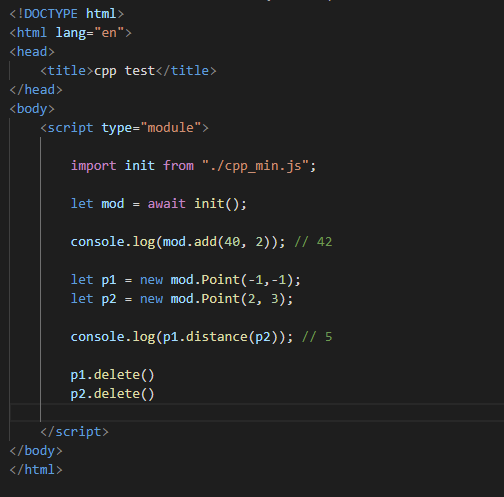
\includegraphics[width=0.50\linewidth]{demo.PNG}
  \caption[loading a plugin]{Cpp-wasm web demo}
  \label{fig:min-cpp-demo}
\end{figure}

\begin{figure}
  \graphicspath{{../../assets/images/6.1.3/}}
  \centering
  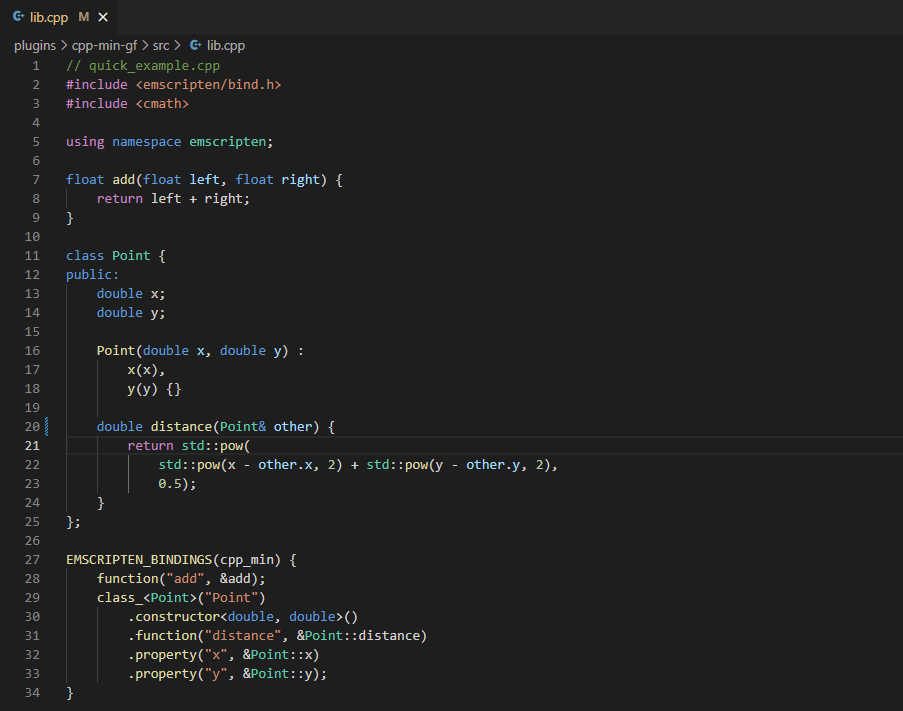
\includegraphics[width=0.50\linewidth]{source.PNG}
  \caption[loading a plugin]{Cpp Plugin Source file}
  \label{fig:min-cpp-source}
\end{figure}

\begin{figure}
  \graphicspath{{../../assets/images/6.1.3/}}
  \centering
  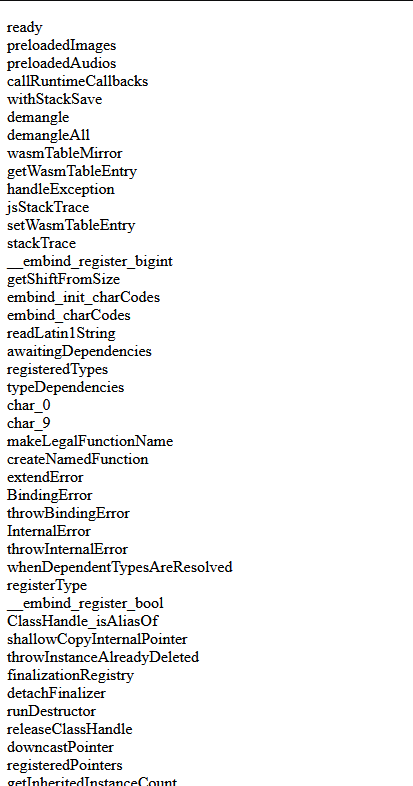
\includegraphics[width=0.50\linewidth]{whitelist.PNG}
  \caption[loading a plugin]{Emscripten JavaScript wrapper blacklist }
  \label{fig:min-cpp-whitelist}
\end{figure}

\subsection{C++: CGAL plugin}

If the minimum cpp plugin example could not be loaded into Geofront, it will be unsurprising that the entirety of CGAL could also not be compiled into a suitable format ready for VPL consumption.
Several steps towards this goal were made however.

A web demo was able to utilize the CGAL kernel \reffig{fig:cgal-tryout-2}, for basic operations. 
Additionally, A subsequent web demo can utilize the CGAL TIN to a limited extend \reffig{fig:cgal-tryout-3}.

However, this study too could not be fully completed within the time frame of this study. 
Two problems prevented completion:

The first one has to do with rewriting inputs and outputs to CGAL functionality.
The most common ways to provide CGAL functions with data, and to retrieve results, is to read and write files. 
While this can be used on the web, the virtual file system wrappers presented by Emscripten add irregular syntax to the plugin, again compromising any chance it can be loaded into Geofront.
So, a way is needed to present CGAL with data directly from javascript or other wasm binaries, without reading or writing files. 
Initial tests were performed by parsing input data as a string buffer, which could then be 'read' like a file by CGAL.

The second issue with this process is to make sure all dependencies, like Boost, are compiled together with CGAL.
Legacy makefile build systems complicate this process. 
To get the current demo's working, several dependencies and sub-dependencies had to be manually traversed, their makefiles had to be edited, and the projects had to be re-compiled and copied to different location, to be used by the emscripten compiler exclusively. 
This is an unsustainable workflow, which will complicate development.  

\begin{figure}
  \graphicspath{{../../assets/images/6.1.4/}}
  \centering
  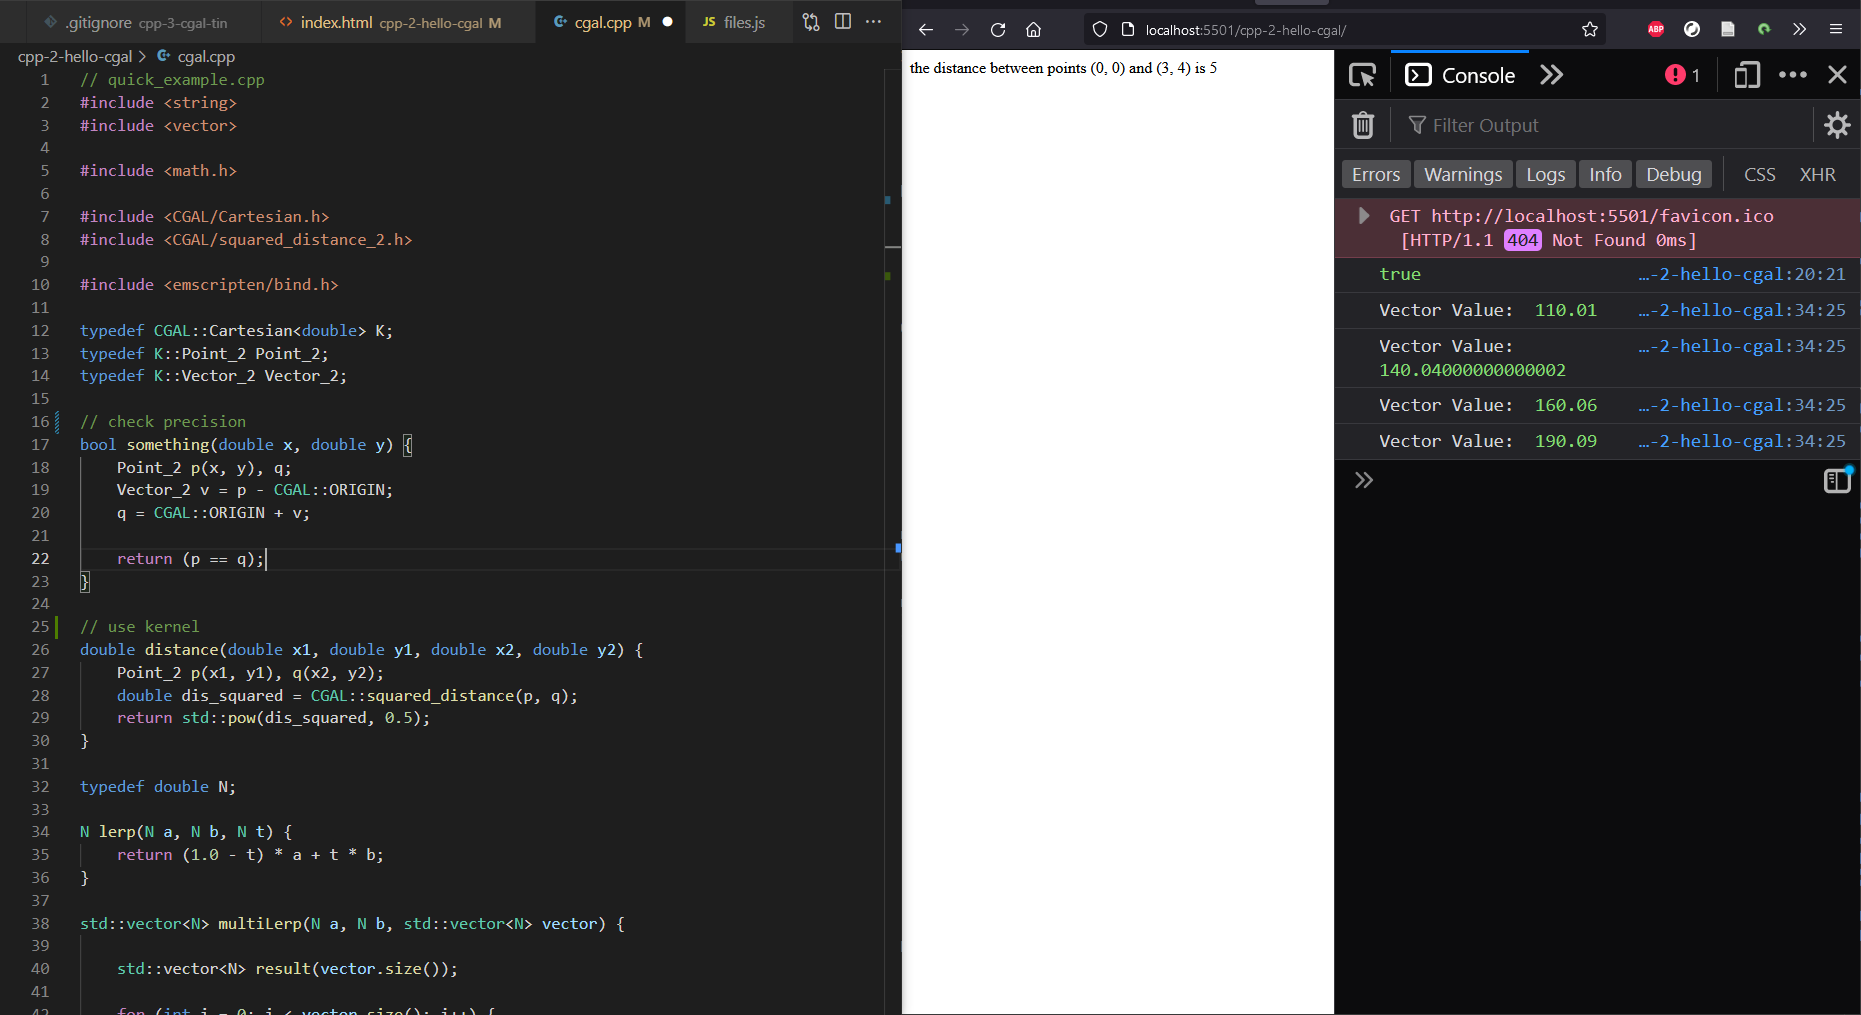
\includegraphics[width=0.50\linewidth]{demo-2.PNG}
  \caption[loading a plugin]{Cpp Plugin Source file}
  \label{fig:cgal-tryout-2}
\end{figure}

\begin{figure}
  \graphicspath{{../../assets/images/6.1.4/}}
  \centering
  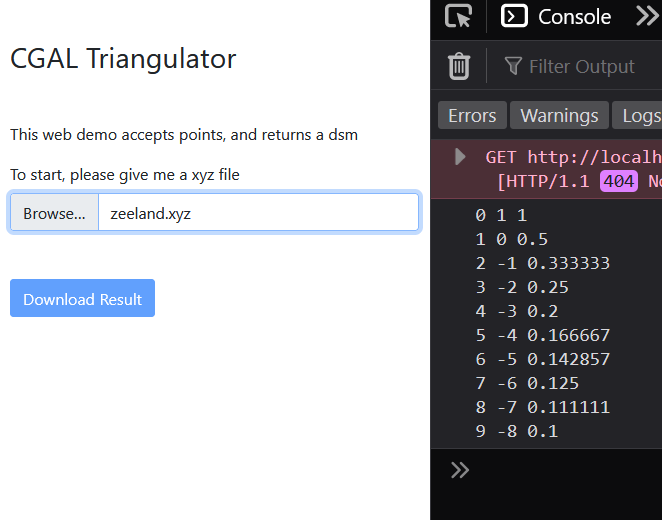
\includegraphics[width=0.50\linewidth]{demo-3.PNG}
  \caption[loading a plugin]{Emscripten JavaScript wrapper blacklist }
  \label{fig:cgal-tryout-3}
\end{figure}

\subsection{Comparison}

\begin{lstlisting}
  combined size of all compiler artifacts produced by wasm-back / emscripten

  wasm-pack:
  rust min:       20140 bytes
  startin:       114263 bytes

  emscripten:
  cpp min:        68424 bytes
  cgal tin test  257994 bytes

\end{lstlisting}

\section{Usability Tests}
\label{sec:testing:usability}

% \subsection{Demo applications}

% - Show a demo

% - Show a bit of performance of said demo

\subsection{Assessment}

This section offers an analysis on the usability of Geofront, according to the framework described by \cite[]{green_usability_1996}.

\subsubsection*{Abstraction gradient: What are the minimum and maximum levels of abstraction? Can fragments be encapsulated?}

Geofront was meant to support encapsulation. 
The need for re-using parts of a script as components / functions was deemed more important than the benefits of having no abstraction hierarchy (what you see is what you get).
An early prototype of Geofront did allow for encapsulation, by taking a subset of a Geofront script, and compiling it to a javascript subset. This could then be loaded by the library loader. 
However, the addition of special types of nodes, and features like iteration, invalidated the \m{geofront -> js} translator.
The translation is still possible, just not implemented.  
As such, if a user desires re-usable components and a lower abstraction level, they will need to write a Geofront library.

% \textbf{Suggestion for improvement:} re-implemented the 'compile to js' procedure.s
% (image of abstracting away a javascript subset)

\subsubsection*{Closeness of mapping: What 'programming games' need to be learned?}

Mapping a problem to a geofront script is intuitive for the most part.
Think of the operations needed to solve a problem, 
find the right libraries and nodes representing these operations,
and connect these nodes according to type. 
However, this mapping of problem and solution is hindered by the fact that Geofront needed to support iteration. 

(image of iteration problem)



\subsubsection*{Consistency: When some of the language has been learnt, how much of the rest can be inferred?}

\cite[]{green_usability_1996} notes on the difficulty of defining 'consistency' in language design, and chose to define it as a form of 'guessability'.

Geofront has introduced certain symbolic distinctions between graphical entities to aid this predictability. 
The biggest is the distinction between \m{operation} and \m{widget} components: 
operations are pure functions with inputs and outputs. 
widgets represent some 'outside world' interaction, like an input value, a file, or a web service. 
This way, 'special behavior' is isolated to widgets, making the rest of the script more predictable. 

In practice, certain inconsistencies within Geofront arise due to the open nature of the plugin system. 
the consistency of geofront is mitigated by a library with a very different notion of naming, or if the library chooses unusual input or output patterns. 
For example, a euclidean, 3D coordinate can be specified as a \m{Vector3} object, a struct, an array of three numbers, or three different x, y, z input parameters.
Then again, it is unclear if inconsistencies between the api's of a language's libraries are to be contributed to the inconsistency of the language as a whole. 

\textbf{Suggestion for improvement:} Stabilize the api of the Geofront Standard Library.



\subsubsection*{Diffuseness: How many symbols or graphic entities are required to express a meaning?}

Geofront periodically suffers from the same 'Diffuseness' problems \cite[]{green_usability_1996} adheres to vpls general. 
That is, sometimes a surprising number of 'graphical entities' / nodes are required to represent a simple statement.  
This is apparent when representing mathematical calculations. 

\begin{note}
  - the flowchart can only represent linear processes. Many geoprocessing algorithms are iterative and make use of conditionals. These cannot easily be expressed in a DAG VPL. As such, these processes must happen within the context of a function, within a 'computational node'  
\end{note}


(image of complex / simple mathematical calcluation in javascript and in geofront)

\textbf{Suggestion for improvement:} These situations could be prevented by allowing scriptable components. 

\subsubsection*{Error- proneness: Does the design of the notation induce 'careless mistakes'?}

There are some errors the user can make  in Geofront that will not be immediately obvious. 
The biggest one is that there are no systems in place preventing large calculations. 
These might freeze up the application. 

To prevent this, the geofront interpreter should have been implemented to run on a separate thread, using a web worker. 
Besides this, in general, many systems are in place preventing errors, such as the type-safety used throughout geofront.
Also, by disallowing cyclical graphs, users cannot create infinite loops accidentally.

\subsubsection*{Hard mental operations: Are there places where the user needs to resort to fingers or pencilled annotation to keep track of what's happening?}

Geofront is developed specifically to prevent "Hard mental operations".
Following the dataflow paradigm explained in \refsec{sec:background:dataflow}, geofront chose to disallows cyclical patterns. 
This greatly reduces the complexity of possible graph configurations, and also causes all in-between results to be immutable or 'final'.
By then allowing these results to be inspected, and allowing the graph to be easily reconfigured, Geofront allows a workflow rooted in experimentation and 'play'.
Users do not need to 'keep track' or 'guess' how things work.
Instead, they can simply experience the behavior, and adjust the behavior until satisfied. 



\subsubsection*{Hidden dependencies: Is every dependency overtly indicated in both directions? Is the indication perceptual or only symbolic?}

The dimension of 'hidden dependencies' is another way the dataflow-paradigm is advantageous. 
The pure functions of a diagram-based vpl like Geofront make the language in general consistent and predictable.
However, there are two exceptions to this rule:
First, the \m{widget} nodes are allowed to produce side-effects, such as opening a window, asking for an input, making a web request, etc. 
These are required to provide geofront with interactive inputs and outputs.
The distinction between \m{widgets} and \m{}

And second, the pureness of functions can only be maintained if all Geofront libraries also exclusively use pure functions. 
There is no fail-safe in place to prevent the usage of a library containing functions with many side-effects. 

\subsubsection*{Premature commitment: Do programmers have to make decisions before they have the information they need?}

In general, Geofront requires almost no premature commitment. 
Or, rather, the level of premature commitment is in line with textual programming languages, in the sense that a user is always somewhat committed to the structure they themselves build. 

One practical way in which Geofront exceeds in this dimension of premature commitment, is that the application does not require a restart upon loading a new library. 
Users can add or remove libraries "on the fly". 
This is unlike any vpl studied at \refsec{sec:related-geovpl} or \refsec{sec:related-webvpl}.

One particular type of commitment users must be aware off, however, is the commitment to using a \ac{VPL} like Geofront. 
Therefore, 


\subsubsection*{Progressive evaluation: Can a partially-complete program be executed to obtain feedback on 'How am I doing'?}

Yes. 
As explained at the answer for the dimension of 'Hard mental operations', this is a core aspect in how Geofront achieves its interactivity and debugability, together with its ability to inspect parameters. 

(Image: Show example)

\subsubsection*{Role- expressiveness: Can the reader see how each component of a program relates to the whole?}

as the authors of \cite[]{green_usability_1996} write: "The dimension of role-expressiveness is intended to describe how easy it is to answer the question 'what is this bit for?'"

sizeable phenomenon

grootste boosdoener: looping is now a simple boolean toggle within a component. 
This makes it very non-explicit, 

This leads to another problem: the problem of declarative iterations within a vpl. 


\subsubsection*{Secondary notation: Can programmers use layout, color, other cues to convey extra meaning, above and beyond the 'official' semantics of the language?}

No, Geofront does not offer annotations in its current state, besides the way the nodes are configured on the canvas.  
Geofront does provide visual indicators for types, and for if a cable / variable represents a single item, or a list of items.

\textbf{Suggestion for improvement:} Provide a way to annotate: create groups, write comments, etc. 
\textbf{Suggestion for improvement:} Type colors would also be nice.

\subsubsection*{Viscosity: How much effort is required to perform a single change?}

Despite these efforts, the 'mouse intensive' interface of vpls like Geofront continues to be a hinder for viscosity.
Certain situations require excessive mouse interaction, like substituting a function with another function, but keeping all inputs the same.
In text, this would be as simple as a non-symbolic renaming of the called function.
In geofront, this requires a lot of reconfiguration of cables. 

\textbf{Suggestion for improvement:} Viscosity could be improved by creating special actions in the editor to perform these types of manipulations.  
%  - select multiple inputs, select multiple outputs: connect by height.
% rename node


\subsubsection*{Visibility: Is every part of the code simultaneously visible (assuming a large enough display), or it it at least possible to juxtapose any two parts side-by-side at will? If the code is dispersed, is it at least possible to know in what order to read it?}

All parts of the code are simultaneously visible. 
As the question implies, by not making the code dispersed, 

% ## Case Studies

% ### Vector
% _Vector data retrieval, transformation, visualization_

% ### Raster 
% _Raster data retrieval, transformation, visualization_

% ### 6. Experiments 
% _Performance benchmark between rust-wasm / cpp-wasm / cgal-cpp-wasm / js / cli usage_

% ## Final 
% _Answer research questions ????_


%%%%%%%%%%%%%%%%%%%%%%%%%%%%%%%%%%%%%%%%%%%%%%%%%%%%%%%%%%%%%%%
%%%%%%%%%%%%%%%%%%%%%%%%%%%%%%%%%%%%%%%%%%%%%%%%%%%%%%%%%%%%%%%
%%%%%%%%%%%%%%%%%%%%%%%%%%%%%%%%%%%%%%%%%%%%%%%%%%%%%%%%%%%%%%%
%%%%%%%%%%%%%%%%%%%%%%%%%%%%%%%%%%%%%%%%%%%%%%%%%%%%%%%%%%%%%%%

% OLD OLD OLD OLD OLD OLD OLD OLD OLD OLD OLD OLD OLD OLD OLD


% We group the requirements listed at \refsec{sec:method-one} in a group of base features,
% a group of dataflow features, and a group of geometry features.


% \section{Experiments}

% \subsection{ Web Mapping Service }
% -> could work, must be captured in component
% -> streaming question

% \subsection{ Open Street Map }
% -> could be hooked up to the geojson viewer



% \section{ Performance }
% \subsection{Vector 3D}

% ....

% \subsection{Raster}

% ....

% \subsection{Geo features}

% ....


%%%%%%%%%%%%%%%%%%%%%%%%%%%%%%%%%%%%%%%%%%%%%%%%%%%%%%%%%%%%%%%%%%%%%%%%%
% \section{Use Case: Educational Sandbox}
% \begin{lstlisting}
% WHAT: 
%  - show the behaviour of a simple ransac algorithm, fitting a plane through 
%    a point cloud
%  - show it beharivourly: show in-between steps
%  - make parameters ajustable (number of high scores, minimum high score, 
%    number of tries, etc.)
%  - add least squares adjustment, and compare.

% SIMILAR EXAMPLES: 
%  - the geometric predicates explanation 
%  (https://observablehq.com/@mourner/non-robust-arithmetic-as-art)
%  - 

% ASSESS ON: 
%  - educational value
%  - ease of usage (the promise of **Criterium A**)
 
% ASSESSMENT (hypothesis): 
%  + indeed very insightful for analying the behaviour 
%    and operation of certain 
%    algorithms & parameters. Not many applications can show 
%    this level of insight. 
%  + feature B can be used to strip the tool down 
%    to the bare minimum,   helping 
%    with not overwhelming the user with features

%  - This VPL is not easy to operate. 
%    It remains difficult to communicate what needs to 
%    be done, how things work. This is not an expert tool, 
%    but also not a beginners' tool.
%  - No built-in tutorialization
%  - hard to discover the code underneath, 
%    obfuscating the link between process and code.

% \end{lstlisting}

% %%%%%%%%%%%%%%%%%%%%%%%%%%%%%%%%%%%%%%%%%%%%%%%%%%%%%%%%%%%%%%%%%%%%%%%%%
% \section{Use Case: Web Demo Environment}
% \begin{lstlisting}
%     WHAT:
%      - Show the startin delaunay triangulator
%      - Accept user-submitted Laz files as input
%        - filter the ground
%      - Accept a randomly generated point cloud based on perlin noise.
%      - Visualize the generated mesh, and make it available for download

%     EXAMPLES: 
%      - hugo's demo
    
%      ASSESS ON:
%      - **Criterium B**: extendability: 
%        - how does foreign and native codebases interact? 
%      - clarity
%      - reproducibility
%      - performance
%      - scope (raster / vector / 2D / 3D)

%     JUDGEMENTS (hypothesis): 
%      + Clarity is fine
%      + Reproducability is 
%      + Performance is decent

%      ~ clarity is fine, vpl allows users to 'play around' and try
%        different configurations, even run their own data through the
%        demonstrated functions

%      - Application is less suited for 2D 
    
% \end{lstlisting}


% \section{Use Case: Geoprocessing Environment}%%%%%%%%%%% SECTION
% \begin{lstlisting}

%     WHAT:
%       - Query an area of a point cloud with a polygon
%       - turn that area of points into a triangulation
%       - turn triangulation into isocurves
%       - save this as a geojson
%       - turn this whole thing into a function, which takes a PC, 
%         polygon and isocurve range, and spits out the geojson
%       - share this using a link
%       - turn this into an app?
%       - turn this into a script?

%     EXAMPLES: 
%      - 

%      ASSESS ON:
%      - **Criterium C**: Publicability:
%        - the ability to operationalize the application 
%        - can it be used by end-users? clarity? too much clutter

%     JUDGEMENTS (hypothesis): 
%       ~ sharing by link is possible, but for end-user usage, 
%         its very cluttered 
%       ~ compiling to js only partially works
%       ~ compiling into an app is not possible, but 
%         since everything runs client-side, it could be implemented. 

% \end{lstlisting}
